\documentclass[12pt, letterpaper]{article}
%\documentclass[12pt, letterpaper, titlepage]{article}

\usepackage{setspace} \doublespacing
\usepackage{amsmath}
\usepackage{booktabs}
\usepackage{amsthm}
\usepackage{graphicx}
\usepackage[margin=1in]{geometry}
\usepackage{hyperref}
\hypersetup{colorlinks = true, linkcolor = blue, citecolor=blue, urlcolor = blue}
\usepackage{enumitem}
\usepackage{setspace}
\usepackage{lipsum}
\usepackage{siunitx}
\usepackage[square,numbers]{natbib}
\bibliographystyle{abbrvnat}



\usepackage[]{lineno}
\linenumbers*[1]


% NOTE: To produce blinded version, replace "0" with "1" below.
\newcommand{\blind}{0}

\setlength{\linewidth}{3in}

\providecommand{\keywords}[1]
{
  \small	
  \textbf{\textit{Keywords---}} #1
}

\begin{document}
%\maketitle

\if0\blind
{
  \title{\bf A Concise Survey on Statistical Analysis in Bike Lane Research}
  \author{Zoe Macris\\
  University of Connecticut}
\date{December 2023}
  \maketitle} 

%\doublespace

\begin{abstract}
This survey paper examines the evolving field of statistical analysis of bicycle lanes. Cycling plays an important role in society, and has taken a place as a sustainable and accessible mode of transportation and exercise. In order for cycling to be accessible for the most number of people, investments into bike lanes and cycling infrastructure have to be made. Through an examination of existing studies, we explore the current trends in method to show whether bike lanes have a statistically significant effect on cycling outcomes. 
\end{abstract}
\label{sec:abstract}

\keywords{Bike Lanes, Regression Analysis, Binary Regression Models, Multiple Level Regression Analysis, Zero-Inflated Poisson, Generalized Linear Model}


\section{Introduction}
\label{sec:intro}

Given that they have been around for just over 200 years, the bicycle has  evolved considerably in it's utility to us as a society. Originally just for hobbyists, and inhibitively expensive, they are now one of the most accessible modes of transport \cite{BIKE2023}. The World Health Organizations recommendation is a minimum of 150 minutes of moderate aerobic activity per week \citep{WHO2020}. This is difficult to achieve in our sedentary society, but cycling is an excellent form of exercise that can also double as the mode of transport for commuting and completing daily tasks. \par
Statistical research and analysis on bike lanes provides crucial insights into the usage patterns, attitudes, commute rates, bicycle traffic and safety. Other survey papers on research into bike lanes have neglected to focus on the statistical analyses used in the research \cite{7Mlenberg2019}. This survey paper aims to provide an comprehensive examination of the existing body of statistical research into bike lines. With this, we hope to show trends in the research, give an overview of statistical findings and identify areas that can be further developed. \par
The rest of the paper will be organized in the following manner. Section \ref{sec:Background} will present a background about bike lanes and why they are important. Section \ref{sec:methodanddata} will present how the survey was conducted. Section \ref{sec:disc} will discuss the findings and recommendations. Then \ref{sec:conc} will conclude the paper.


\section{Background}
\label{sec:Background}

In order to understand the research into bike lanes, these topics should be understood. 

\subsection{Benefits of Cycling}
\label{sec:benefit}

According to \citet{Gtschi2015}, getting the appropriate amount of exercise has an estimated risk reduction of 30\% for all-cause mortality, including from cardiovascular disease, coronary heart disease, stroke, diabetes and cancer . It also can help people's mental health as well as physical, some studies have even demonstrated a decrease in depression symptoms from cycling for transportation \cite{Green2021}. \par
Beyond these individual benefits, cycling has a benefit for the environment and society as a whole. Transportation is a large source of greenhouse gas emissions for many countries \cite{Green2021}. In recent years, there has been even more emphasis on sustainable and environmentally conscious transportation options in urban areas. Cycling fits the these criteria and has risen to prominence as a viable sustainable mode of transportation. It is a form of active transportation, which is defined as human powered, and thus does not release greenhouse gas emissions. Bikes also take up considerable less space and require significantly less infrastructure than cars as an added benefit.\par 
In order to promote cycling and make use of the benefits of alleviating traffic congestion, reduced emissions, and enhancing public health, it is necessary to plan and evaluate cycling infrastructure, and bike lanes more specifically. Statistical analysis can come into play here and help prove whether bike lanes make a significant impact on the propensity of people cycling and their safety while doing it. 

\subsection{Types of Infrastructure}
\label{sec:bikeshare}

The Connecticut State government describes the common facility types used to accommodate cyclists as Shared Roadways (Informal On Road), Wide Curb-lanes, Bicycle Lanes and Multi-use Paths. The visuals in Figure ~\ref{fig:bikelane}, show an even wider array of potential infrastructures. In the U.S., commonly seen types are Bicycle Awareness Zones, Informal On Road and Bicycle Lanes as seen in the images. The supposition of much of the research analyzed here is that the more advanced the infrastructure is, the more likely people are to cycle \cite{1MateoBabiano2016}.\par 

\begin{figure}[hbt!]
    \centering
    \includegraphics[width=0.75\textwidth]{Bikelane.jpg}
    \caption{Bike Lane Comparison \cite{1MateoBabiano2016}}
    \label{fig:bikelane}
\end{figure}

Shared roadways are where bicycle and automobile travel are allowed, all streets and roads other than controlled highways, are in this category. They do not provide any added protection to cyclists, but a street's designation as shared roadway indicates to cyclists that there are advantages to using the route over alternatives \cite{CTDOT2023}. \par 
Wide curb lanes are still require sharing between bicycle and motorized traffic, but they provide more distance between bicyclists and vehicles and protection from high traffic speeds. They are created by widening roadways or narrowing traffic lanes, or both \cite{CTDOT2023}.\par 
The category of bicycle lanes is defined as painted and signed lanes on the shoulder of streets, to improve conditions for bicyclists and to protect them from traffic volume and speed. Being designated as a bike lane street, means that more "pavements surface improvements, stronger sweeping programs, special signal facilities, etc" occur on them to increase safety and comfort for cyclists \cite{CTDOT2023}. \par
The last level of cycling infrastructure is multi-use paths, on which cyclists have exclusive rights-of-way and don't cross The flow of automobiles more than necessary. These can be both recreational opportunities or high=speed commuter routes for cyclists \cite{CTDOT2023}. \par
The research in this survey focuses on the infrastructure of bicycle lanes, and whether they are sufficient to increase the propensities of people to cycle, and their safety while they are cycling. 


\section{Method and Data}
\label{sec:methodanddata}

To conduct this comprehensive survey of statistical analyses on bike lanes, a search was conducted of academic databases such as Science Direct, ProQuest, MDPI, and PubMed. These searches were conducted through the University of Connecticut library of Databases to ensure they were papers that were a able to be accessed. Specific terms were used including "bike lane", "statistical analysis", and "cycling infrastructure" in order to identify relevant papers. The date range for literature was defined as 2012 to the present, upon evaluation of typical date range of the available literature. \par

\subsection{Criteria of Inclusion and Exclusion}
\label{sec:inc}

Literature was included in the survey if it met these criteria:

\begin{enumerate}
        \item Whether the paper held sufficient statistical analysis on the topic of bike lanes. 
        \item Being publicized in a peer-reviewed, reputable journal.
        \item Availability of paper for access using University of Connecticut student status. 
\end{enumerate}

\subsection{Data}
\label{sec:data}

The data in this survey paper is the types of statistical analyses conducted by the identified literature from method given above. A selection of eleven papers resulted from this, and the approach used to identify relevant data from the papers to be discussed in the survey paper was done as follows. The specific type of statistical analysis conducted in the paper was identified. Alongside the method and variables used by the researchers in the study. The results from the data collection are displayed in ~\ref{sec:results}. 

\section{Results}
\label{sec:results}

\subsection{Correlation and Regression Analysis}
\label{sec:corr}

The correlation and regression analysis approach of statistical research on bicycle lanes is used to establish significant relationships amongst variables. In \citet{1MateoBabiano2016}, the approach using Spearman's correlation coefficient rho was used, which was suitable because the variables deviated from a normal distribution. The variables used were Public bicycle-sharing programs (PBSP) station usage frequency and length of bike-ways, which do not follow a normal distribution. The results of the Spearman correlation of station usage and infrastructure type can be seen in ~\ref{table:MB}, where shred pathways, bicycle paths, connections, and separated pathways were shown to have a significant impact on PBSP usage. \par
Other analyses used include Differences-in-Differences, Pearson's R correlation coefficient, Panel regressions, and Counterfactual based on control \cite{Karpinski2021}. These were used when the data being analyzed was usership of Boston's bike share program before and after the addition of bike lanes. 



\begin{table}[tbp]
\small
\label{table:MB}
\centering
\caption{Length of bikeway by bikeway type in Brisbane and CityCycle areas. Spearman correlation of station usage and infrastructure type: from Mateo-Babiano paper}
\begin{tabular}{l*{5}{p{1.5cm}}}
\toprule
{Infrastructure type} & {Length Brisbane Area (km)} & {Lenth in CityCycle area (km)} & {Correlation coefficent} & {P-value}\\
\midrule
Shared Pathway & 327.9 & 18.0 & 0.42 & <0.01 \\
Bicycle Lane & 186.7 & 21.3 & 0.03 & 0.69 \\
Bicycle Awareness Zone (BAZ) & 303.7 & 40.3 & -0.07 & 0.39 \\
Bicycle Path & 23.9 & 2.6 & 0.27 & <0.01 \\
Bicycle Route (BAZ) & 76.9 & 8.2 & 0.13 & 0.11 \\
Connect & 19.5 & 5.0 & 0.16 & 0.049 \\
Informal Off Road & 65.8 & 4.6 & 0.00 & 0.98 \\
Informal On Road & 18.2 & 4.1 & -0.13 & 0.12 \\
Separated Pathway & 1.8 & 1.3 & 0.29 & <0.0 \\
\bottomrule
\end{tabular}
\end{table}


\subsection{Binary Regression Models}
\label{sec:bin}

In the paper by \citet{2Yujun2019}, binary probit regression analysis was used to analyze the choice of cycling for commuting, since the dependent variable to choice to bicycle to commute has two outcomes:

\begin{itemize}
    \item 0, the individual does not commute by cycling.
    \item 1, the individual commuted by cycling at least once per week.
\end{itemize}
    
For the binary model, a latent or unobserved variable y* is assumed that ranges from $\infty$ to $-\infty$, which is related to the independent variable by the equation $y^{*}_{i} = x_{i}\beta + \epsilon_{i}$. In the context of this survey paper, this latent variable are what underlies the decision making process of bicycle commuting. Where $X_{i}$ is a matrix of independent variables and $\beta$ is a vector of coefficients to be estimated and $\epsilon$ is random error \cite{LONG2001}. 

The binary logistic regression model is also used in this field of statistical research to predict the likelihood of a successful event occurring, like a high number of cycling routes close to green areas \cite{5CamposSnchez2019}. Binary logistic regression serves as an indispensable tool in predictive modeling due to its versatile applications and tailored approach to analyzing binary dependent variables. Unlike linear regression, which is suitable for predicting continuous values, binary logistic regression is specifically designed for situations where the outcome is dichotomous, such as survival vs. death, presence vs. absence, or default vs. non-default in loan scenarios. In the case of \citet{5CamposSnchez2019}, multiple variables are coded 1-0 in a binary fashion and can be seen in Figure ~\ref{fig:vartable}. \par
\begin{figure}[hbt!]
    \centering \includegraphics[width=1\textwidth]{vartable.png}
    \caption{Variable Table for Binary Logistic Regression Model}
    \label{fig:vartable}
\end{figure}

One of the prime reasons for favoring binary logistic regression over linear regression for binary outcomes is the inherent nature of the dependent variable. In logistic regression, the model predicts the probability that the dependent variable will assume a value of 1. This probability is modeled using a logit function, ensuring the estimation of the relationship between independent variables and the probability of the event occurring.

The logistic regression model itself relies on statistical estimation methods, primarily the maximum likelihood estimation. This method aids in determining the coefficients of the model, such as 'B0' to 'Bk', which correspond to the influence of each independent variable on the log odds of the binary outcome. These coefficients are estimated using iterative algorithms like Fisher scoring or the Newton-Raphson method, allowing for practical implementation using programming languages like R or Python \cite{Penman_2022}.

\subsection{Multiple Level  Regression Analysis}
\label{sec:mult}

The paper from \citet{3Teixeira2020} uses Multiple Level Logistic Regression to analyze the impact of cycling in various cities with different cycling infrastructure on stress markers. This analysis resulted in the data shown in Figure ~\ref{fig:stress}, of stress levels measured in different cities. The results of this research found that riding on a protected bike lane significantly reduces cyclists stress levels compared to cycling on the general use street.
\begin{figure}[hbp!]
    \centering
    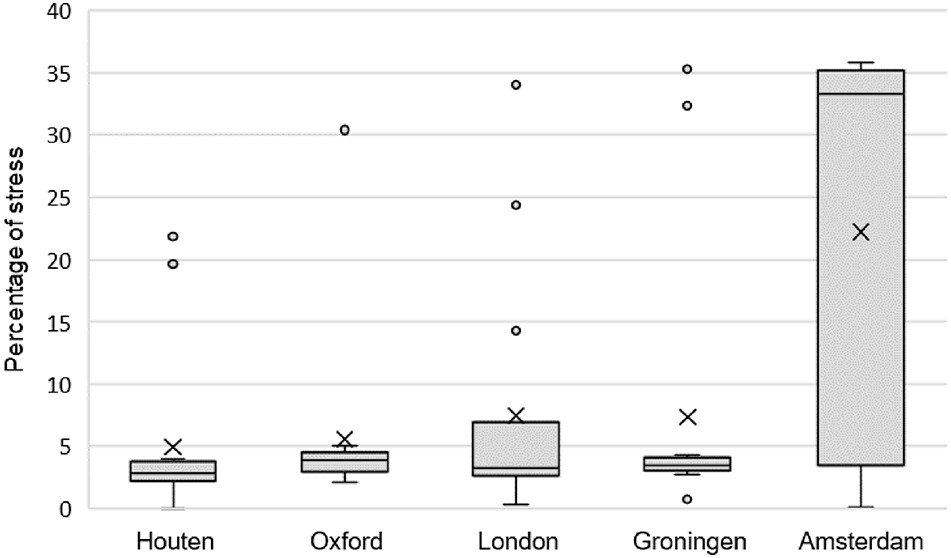
\includegraphics[width=0.5\textwidth]{stresstable2.jpeg}
    \caption{Distribution of Stress by City from Teixeira Study}
    \label{fig:stress}
\end{figure}

Two types of models were used in \citet{4Buehler2011}, a log-log Ordinary Least Square (OLS) model "with the dependent variable being the bike commuters per 10,000 population. As well as a Binary Logit Proportional model "with the share of bike commuters in each city as the dependent variable". This paper analyzed the role of cycling infrastructure on commutership by bike in 90 of the largest 100 U.S. cities. The OLS model is used for estimating coefficients of linear regression that describe the relationship between one or more quantitative independent variables and a dependent variable \cite{XLSTAT2023}. With p explanatory variables, the OLS regression model is: 
\[Y = \beta_{0}+\sum_{j=1,\dots, p}{\beta_{j}X_{j}}+\epsilon\]

In the group of papers addressed, the multinomial logit (MNL) model was used to estimate the travel choice of bicycle for commuting \cite{10Zhao2013}. 

\subsection{Zero-inflated Poisson Regression Mode}
\label{sec:pois}

A different approach that was used in the research into bike lanes was to use a zero-inflated Poisson regression model to estimate the change in cycle-motor vehicle collisions \cite{8Bhatia2016}. This model is used since the design is looking at collision rates pre to post instillation of bike lanes, and since the model allows for an over-abundance of zero counts in the data \cite{Giles2010}. The Poisson distribution's p.m.f is:
\[P(Y=y) = \exp{(-\lambda)\lambda^{y}}/y!\]

The Poisson model is also used in \citet{9Cantisani2021} to "address the randomness due to the perception and decision of road users at the intersections", as their research is specifically on the crash likelihood of cyclists at roundabouts with different infrastructure types. 

\subsection{Generalized Linear Model}
\label{sec:gen}

The final method identified from the surveyed papers was to use the generalized linear model (GLM) to predict the vehicle delays caused by bicycle traffic versus other variables. The GLM has the benefit of being able to accommodate various types of response variables, including continuous, binary, count, and categorical data. It allows for different types of probability distributions such as Gaussian, Poisson, Binomial, etc., making it applicable in a wide range of scenarios. Additionally, GLMs are not restricted to normality assumptions, which makes them suitable for data that is distributed non-normally \cite{PennState2023}.

Alongside this method, the cumulative curve method as used to extract traffic flow data from videos \cite{6Pu2017}. The basic model of the generalized linear model is:
\[Y_{nx1} = X_{nxp}\beta_{px1}+\epsilon_{nx1}\]
Where the matrix of observed values of dependent variables is  $Y_{nx1}$, $X_{nxp}$ is the matrix of observed explanatory variables, $\beta_{px1} =$ is the matrix of coefficients for explanatory variables, and $\epsilon_{nx1}$ is the error. Using this model is reported to help to understand how each factor contributed to the delay of cyclists on urban streets. In Figure ~\ref{fig:traffic}, the results are shown of results of the significance of multiple variables on vehicle delay, and it can be seen that with this method, bicycle and vehicle flow as well as the number of vehicle lanes, has a significant effect on vehicle delay. The results of flow vs. density are also shown in Figure ~\ref{fig:flow}, and reveals that the average bicycle speed decreases slightly as the density increases while  the flow is still increasing, and  when there is high density the variation of bicycle speed decreases a great deal. These results are also consistant across multople locations of urban streets. 
\begin{figure}[hbt!]
    \centering 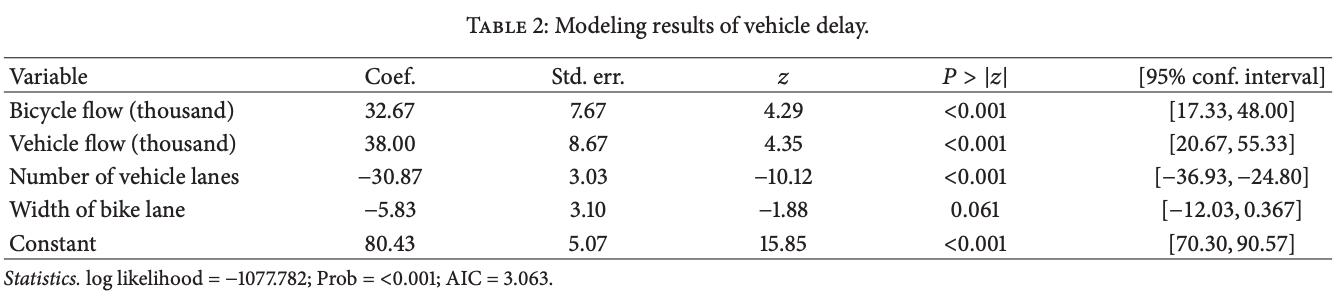
\includegraphics[width=1\textwidth]{BikeTrafficResults.png}
    \caption{Results table from Research on Bicycle Traffic from Pu et al.}
    \label{fig:traffic}
\end{figure}

\begin{figure}[hbt!]
    \centering 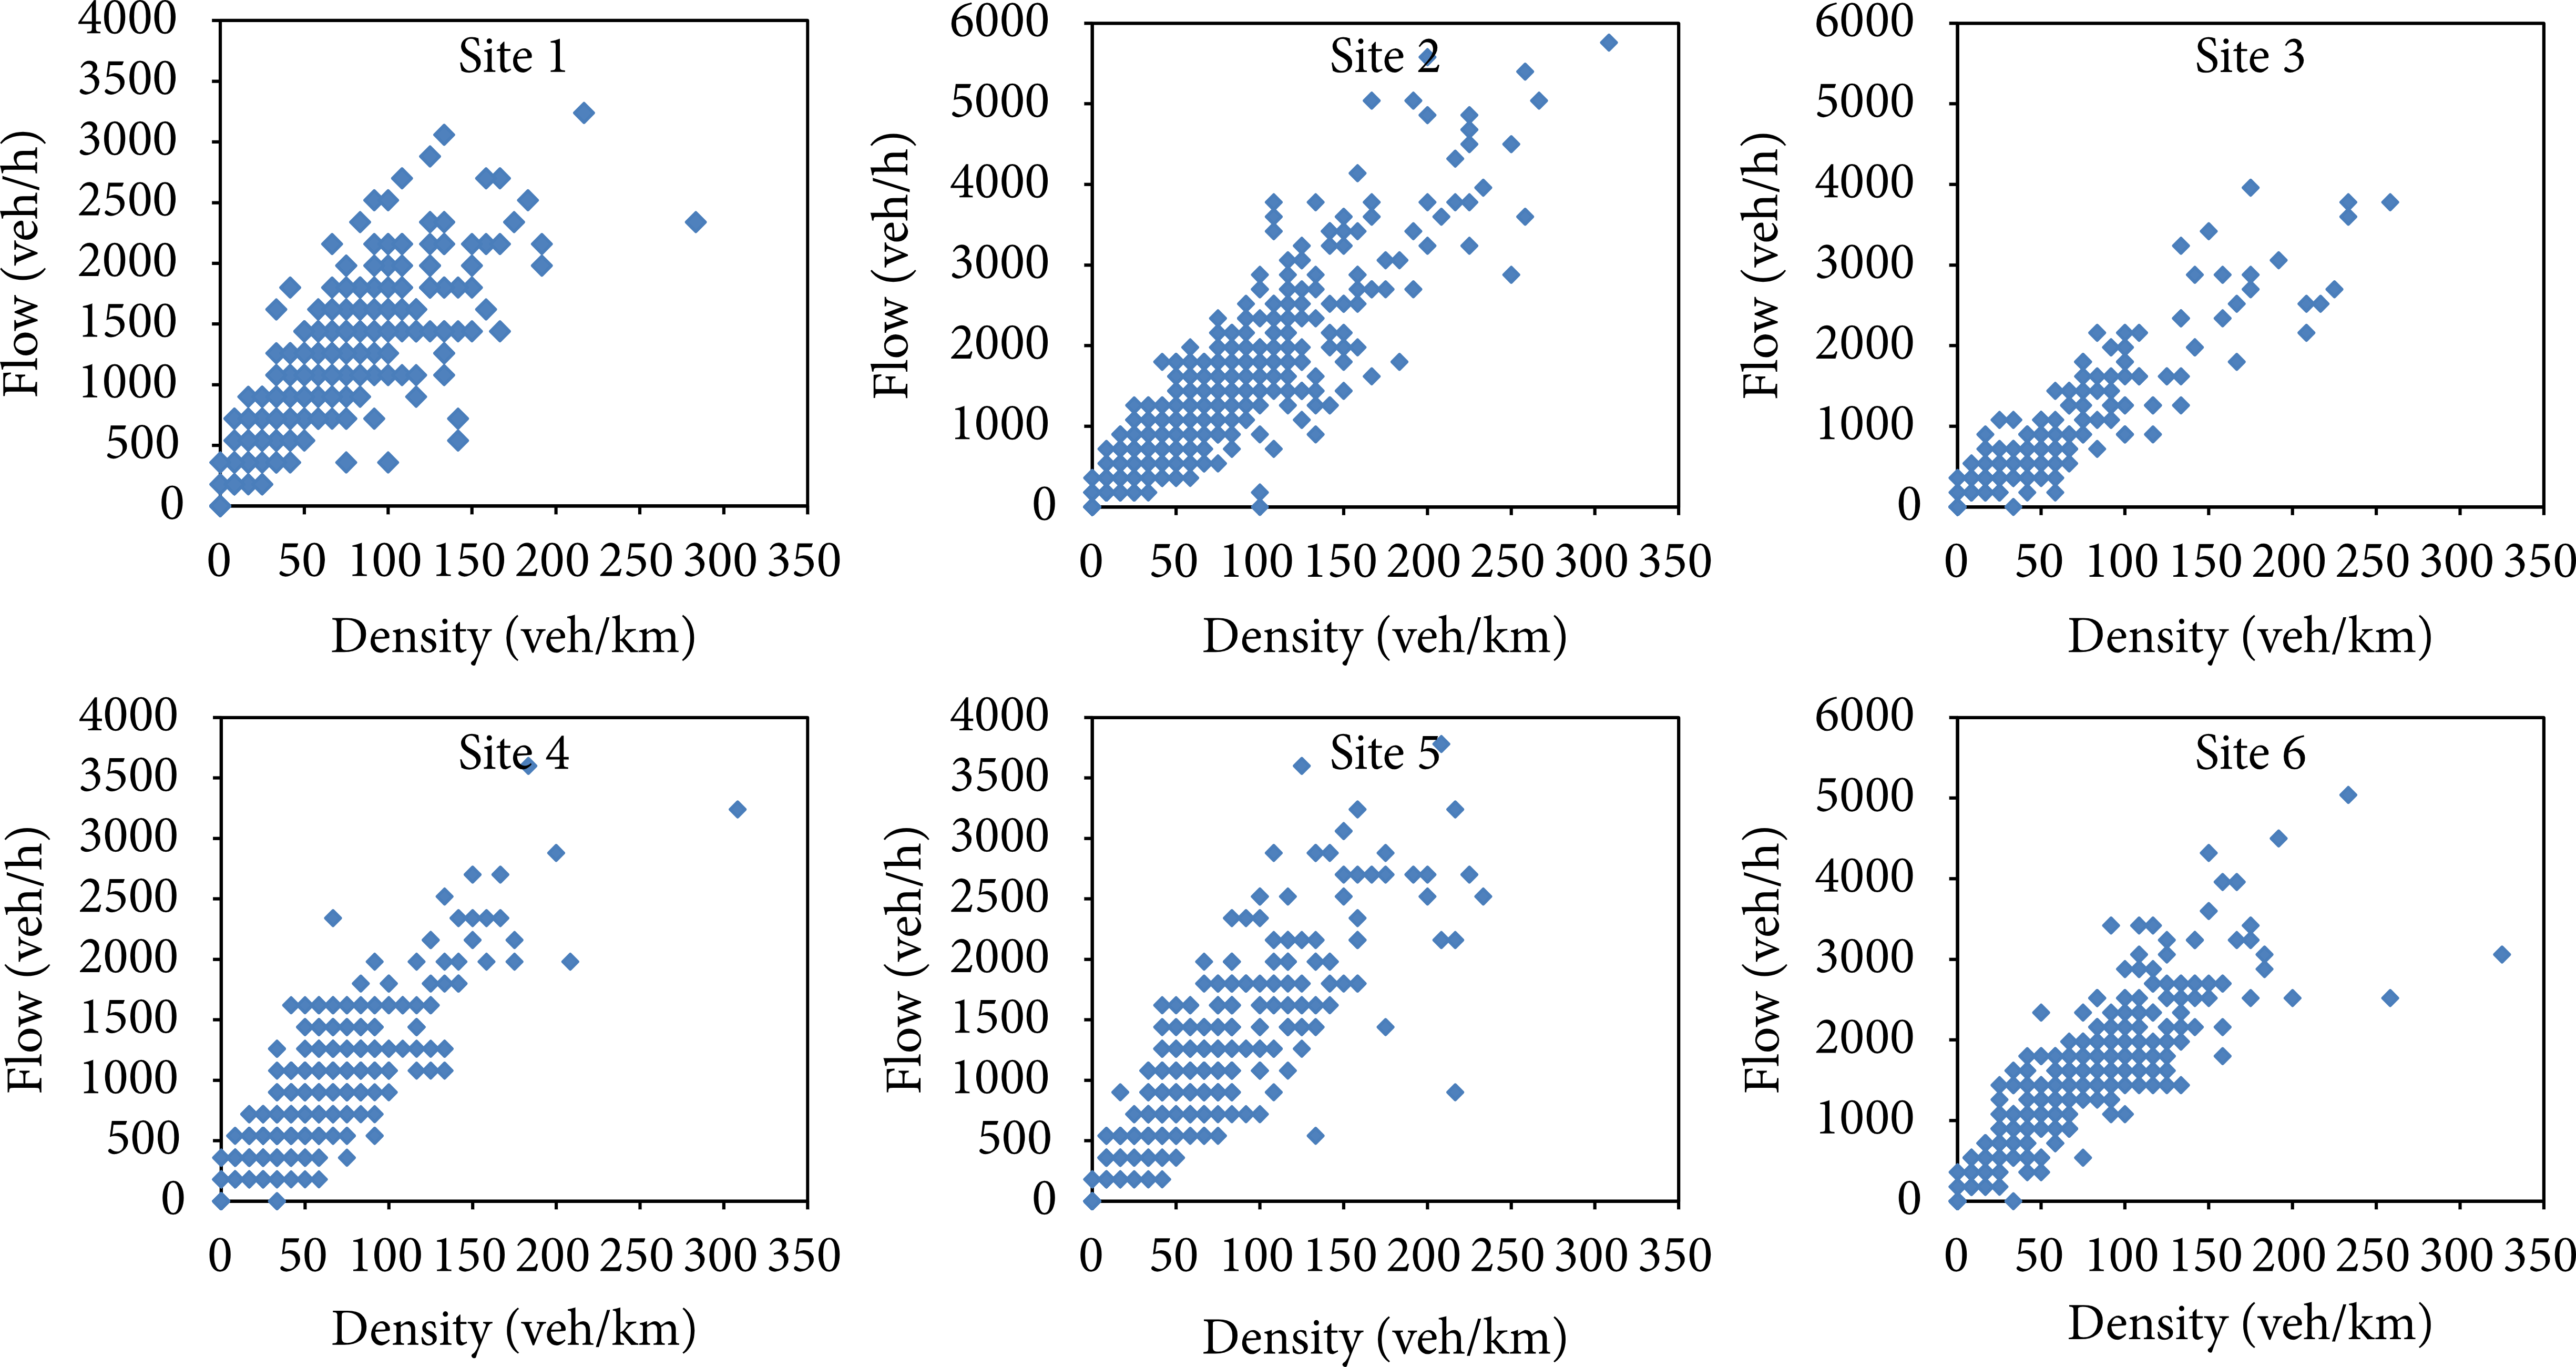
\includegraphics[width=1\textwidth]{flowdensity.png}
    \caption{Relationship between bicycle flow and density}
    \label{fig:flow}
\end{figure}


\section{Discussion}
\label{sec:disc}

The findings from this survey paper show the multifaceted approaches being taken in the field of research into cycling infrastructure, and how important they are to encourage sustainable urban transportation. In this discussion section will include; key themes, criticisms, and potential future pathways for similar research. \par

The different types of cycling infrastructure, especially bike lanes, are shown in this body of research to have a significant impact on increasing cycling ridership. Whether it's an increase in bike-shares or commutership, this relationship is shown in the papers. This is essential when it comes to appealing to policy makers and decision makers in communities to convince them to add cycling infrastructure to their area. Statistical analyses are influential in providing actionable insights, including the correlation between infrastructure types existing in an area and increased cycling. \par

Studies like \citet{1MateoBabiano2016} show how effective simple methods like Spearman's correlation coefficient can be at revealing the impact of bike lanes on PBSP usage. These sorts of results can lead to insights for urban planners when it comes to designing cities. \par

Predictive models were also used, like binary regression models in \citet{2Yujun2019} to provide insight into all the factors influencing an individuals' choice to cycle for commuting. These predictive models offer ways for policy makers to encourage cycling as a successful commuting option in their cities.\par

Some future directions this field could go include focusing on more that just high socioeconomic areas. This type of research has only really been done in affluent countries, likely because a lot of the research has been based off of bike-share systems. Which leads into another point of improvements, where there could be better ways of collecting data on cyclists, as they are often excluding people who own their own bikes from the data. Additionally, there is room for more cost-benefit analyses on the economic impact of investing in cycling infrastructure. When you create such infrastructure, there could be less congestion and damage to the automobile infrastructure. Which would be beneficial to persuading policy makers towards creating more bike lanes and encouraging cycling. 


\section{Conclusion}
\label{sec:conc}

In conclusion, this survey of statistical research on bike lanes offers a current snapshot of frequently used methods in the analysis of bike lanes. The significance of bike lanes in increasing cycling highlights the need for continued research and innovative statistical analysis to understand how to overcome the challenges of congestion, safety, and sustainability in transportation. This supports the efforts of enhancing cycling infrastructure for the benefits of individuals experiences while cycling and the betterment of entire communities. 


\section{Acknowledgements}
\label{sec:acknow}

I would like to express my appreciation to Professor Jun Yan for his guidance in creating this paper. 

\bibliography{Citations}

\end{document}
%%% LocalWords: nonparametric semiparametric autocorrelation ARMA
%%% Local Variables:
%%% mode: latex
%%% TeX-master: t
%%% ispell-personal-dictionary: ".aspell.en.pws"
%%% fill-column: 80
%%% eval: (auto-fill-mode 1)
%%% End: